\documentclass[12pt,a4paper]{article}

% Essential packages
\usepackage[utf8]{inputenc}
\usepackage[T1]{fontenc}
\usepackage{amsmath,amsfonts,amssymb}
\usepackage{graphicx}
\usepackage{float}
\usepackage{cite}
\usepackage{url}
\usepackage{hyperref}
\usepackage{geometry}
\usepackage{setspace}
\usepackage{titlesec}
\usepackage{caption}
\usepackage{subcaption}
\usepackage{booktabs}
\usepackage{siunitx}
\usepackage{lineno}

% Page setup
\geometry{
    a4paper,
    margin=2.5cm,
    top=3cm,
    bottom=3cm
}

% Line spacing
\doublespacing

% Line numbers (uncomment if required by journal)
% \linenumbers

% Section formatting
\titleformat{\section}{\large\bfseries}{\thesection.}{1em}{}
\titleformat{\subsection}{\normalsize\bfseries}{\thesubsection.}{1em}{}

% Figure and table captions
\captionsetup{font=small,labelfont=bf}

% Hyperlink setup
\hypersetup{
    colorlinks=true,
    linkcolor=black,
    citecolor=blue,
    urlcolor=blue
}

% Title page information
\title{\textbf{The impact of forest management on the temperature sensitivity of SOC decomposition in a forest gradient from mediterranean to boreal}}

\author{
    First Author\textsuperscript{1,2}*, 
    Second Author\textsuperscript{1}, 
    Third Author\textsuperscript{3}\\
    \\
    \textsuperscript{1}Department of [Department], [University Name], [City, Country]\\
    \textsuperscript{2}[Second Affiliation if applicable]\\
    \textsuperscript{3}[Third Institution]\\
    \\
    *Corresponding author: email@institution.edu
}

\date{}

\begin{document}

\maketitle

\begin{abstract}
\noindent
\textbf{Background:} Provide context and rationale for your study. Briefly explain the problem or gap in knowledge that your research addresses.

\textbf{Methods:} Summarize your experimental design, key methods, and analytical approaches used in the study.

\textbf{Results:} Present the main findings of your research, including key quantitative results and statistical significance where applicable.

\textbf{Conclusions:} State the main conclusions and their broader implications. Highlight the significance of your findings and potential applications.

\textbf{Keywords:} keyword1, keyword2, keyword3, keyword4, keyword5
\end{abstract}

\newpage

\section{Introduction}


\subsection{Background and Rationale}


\subsection{Objectives and Hypotheses}

Clearly state your research objectives and hypotheses. For example:
\begin{itemize}
    \item \textbf{Primary objective:} To investigate the relationship between X and Y
    \item \textbf{Secondary objectives:} To evaluate Z and assess W
    \item \textbf{Hypothesis:} We hypothesize that X will significantly affect Y under conditions Z
\end{itemize}






\section{Materials and Methods}

\subsection{Holisoils project introduction}

HoliSoils - Holistic management practices, modelling and monitoring for European forest soils, is an EU funded project (Horizon 2020, Grant Agreements number 101000289), completed in October 2026, with the main aim to develop a harmonised soil monitoring framework.\\
More specifically, the project aimed at developing a consistent knowledge framework of  soil properties, processes, biodiversity and soil microbiota activity, in connection with soil-based ecosystem services (wood production, reduction of greenhouse gas emissions, water supply, soil nutrient retention, avoidance of land degradation), particularly in connection with different management approaches.
Modeling was another of the focuses, specifically improving current models and harmonise them into a monitoring framework for estimating ecosystem fluxes. Directly connected with the modeling activity, the project developed a set of standardised sampling and monitoring protocols shared among all actors for greenhouse gas (GHG) reporting. These were used across multiple sampling campaigns across three consecutive years in different locations over Europe, and results have been collected in a comprehensive database of GHG measurements together with additional edaphic and ecological variables.

\subsubsection{Actors and nations involved}
The project involved a consortium of 20 project partners, 18 from EU and partners from South America (Uruguay) and Asia (Japan):
\begin{itemize}
\item Natural Resources Institute Finland (Luonnonvarakeskus), Luke, Finland
\item Institute of Microbiology of the Czech Academy of Sciences (Mikrobiologický ústav AV ČR, v. v. i.), IMIC, Czech Republic
\item French National Centre for Scientific Research (Centre National de la Recherche Scientifique Research institute), CNRS, France
\item Johann Heinrich von Thünen Institute (Johann Heinrich von Thünen-Institut Research institute), TI, Germany
\item Basque Centre for Climate Change (Asociacion BC3 Basque Centre for Climate Change Klima Aldaketa Ikergai), BC3, Spain
\item Vrije University Amsterdam (Stichting VU University), VU, Netherlands
\item European Forest Institute, EFI, Finland
\item Wageningen Research Foundation (Stichting Wageningen), WR, Netherlands
\item International Soil Reference & Information Centre (Stichting International Soil Reference & Information Centre), ISRIC, Netherlands
\item Stockholm University (Stockholms Universitet), SU, Sweden
\item Transylvania University of Brașov (Universitatea Transilvania din Brașov), UTBV, Romania
\item University of Barcelona (Universitat de Barcelona), UB, Spain
\item University of Aberdeen (The University Court of The University of Aberdeen), UNIABDN, UK
\item Vytautas Magnus University (Vytauto Didziojo universitetas), VMU, Lithuania
\item Aix-Marseille University (Aix-Marseille Université), AMU, France
\item Technical University of Munich (Technische Universität München), TUM, Germany
\item Technical University in Zvolen (Technická univerzita vo Zvolene University), TUZVO, Slovakia
\item Forest Science \& Technology Centre of Catalonia (Centre de Ciència i Tecnologia Forestal de Catalunya), CTFC, Spain
\item National Institute for Agricultural Research (Instituto Nacional de Investigación Agropecuaria), INIA, Uruguay
\item Forestry \& Forest Products Research Institute, FFPRI, Japan
\end{itemize}


\subsubsection{The greenhouse gas management effort and how it connects to other parts of the project}




\subsection{Sites and study design}

\subsubsection{Sites and treatments}

\paragraph{Trenching}
In most sites all treatments have both control and trenched subtreatments. The aim of the trenching is to remove all autotrophic respiration from the total soil respiration. Threnching areas were established (on an area of approximately 2 square meters) by digging trenches at a depth of approximately 30-40 cm and then placing root exclusion fabric around the trenched area. The fabric had around 50 μm mesh size, which prevents roots but allows mychorrizae to penetrate the area, as well as water.

\subsubsection{Sampling}
Soil CO$_2$ from control and trenched locations was measured approximately every second week with closed chambers and gas concentration analyzers (see \ref{par:devices}), basing the flux estimate on the linear regression of the concentration increase over time.
Measurement points for the soil chambers have been established with metal or plastic collars, or in some cases (organic soils) by installing the chamber deeper into the soil, to ensure that there was not air flow between the chamber and the atmosphere.

\paragraph{Devices}\label{par:devices}


\paragraph{Covariates}
Soil temperature and in some cases moisture have been recorded in the upper layer (5-10 cm) with various commercially available sensors.





\subsection{The database}

\subsubsection{Organization of the published dataset}
The database is published as a static resource on Zenodo (ADD LINK HERE!!!!!!!).

The dataset is structured in folders, each corresponding to one site. Inside each folder, there are subfolders corresponding to the measurement series. Each mesurement series is a sampling caimpaign, during which each instrument was started and run several sampings of multiple plots.
Inside each series subfolder there are Apache feather files corresponding to each single measurement. 
Apache Feather is an open columnar binary file format designed for fast data interchange between different programming languages, particularly Python and R. It provides efficient serialization and deserialization of dataframes with minimal overhead, 
which makes it ideal for storing a large number of relatively small files.\\

Each feather file, so each measurement, is associated to a line in the metadata file in each site folder. This contains also the respiration fluxes estimated automatically. The estimates were in some cases trimmed manually by the uploading operators, who selected the window in the time series on which to perform the regression to calculate the fluxes. In other cases, when the operator did not select a manual trimming window, the trimming was done automatically.
The metadata files are then collected together in one single general file in the root folder of the dataset ("All_sites.csv"), where the analyses in this study were performed.\\

The dataset is distributed with both calculated flux values and raw measurements in case the user of the database would want to develop own flux estimation approaches.

\subsubsection{Automatic trimming logic}
Jani to write this.


\subsubsection{Descriptive analysis of the data}


\paragraph{Recoding of the treatments}


\subsection{Modeling SOC decomposition dependency on climate}

Provide detailed protocols that would allow others to reproduce your work. Use subsections for different experimental approaches:




\subsection{The model}

\subsubsection{The Bayesian framework}

\subsection{Implementation and hardware}




\section{Results}

\subsubsection{Descriptive analysis}

\paragraph{Soil respiration and temperature}
% CO2 vs temperature
\begin{figure}[H]
    \centering
    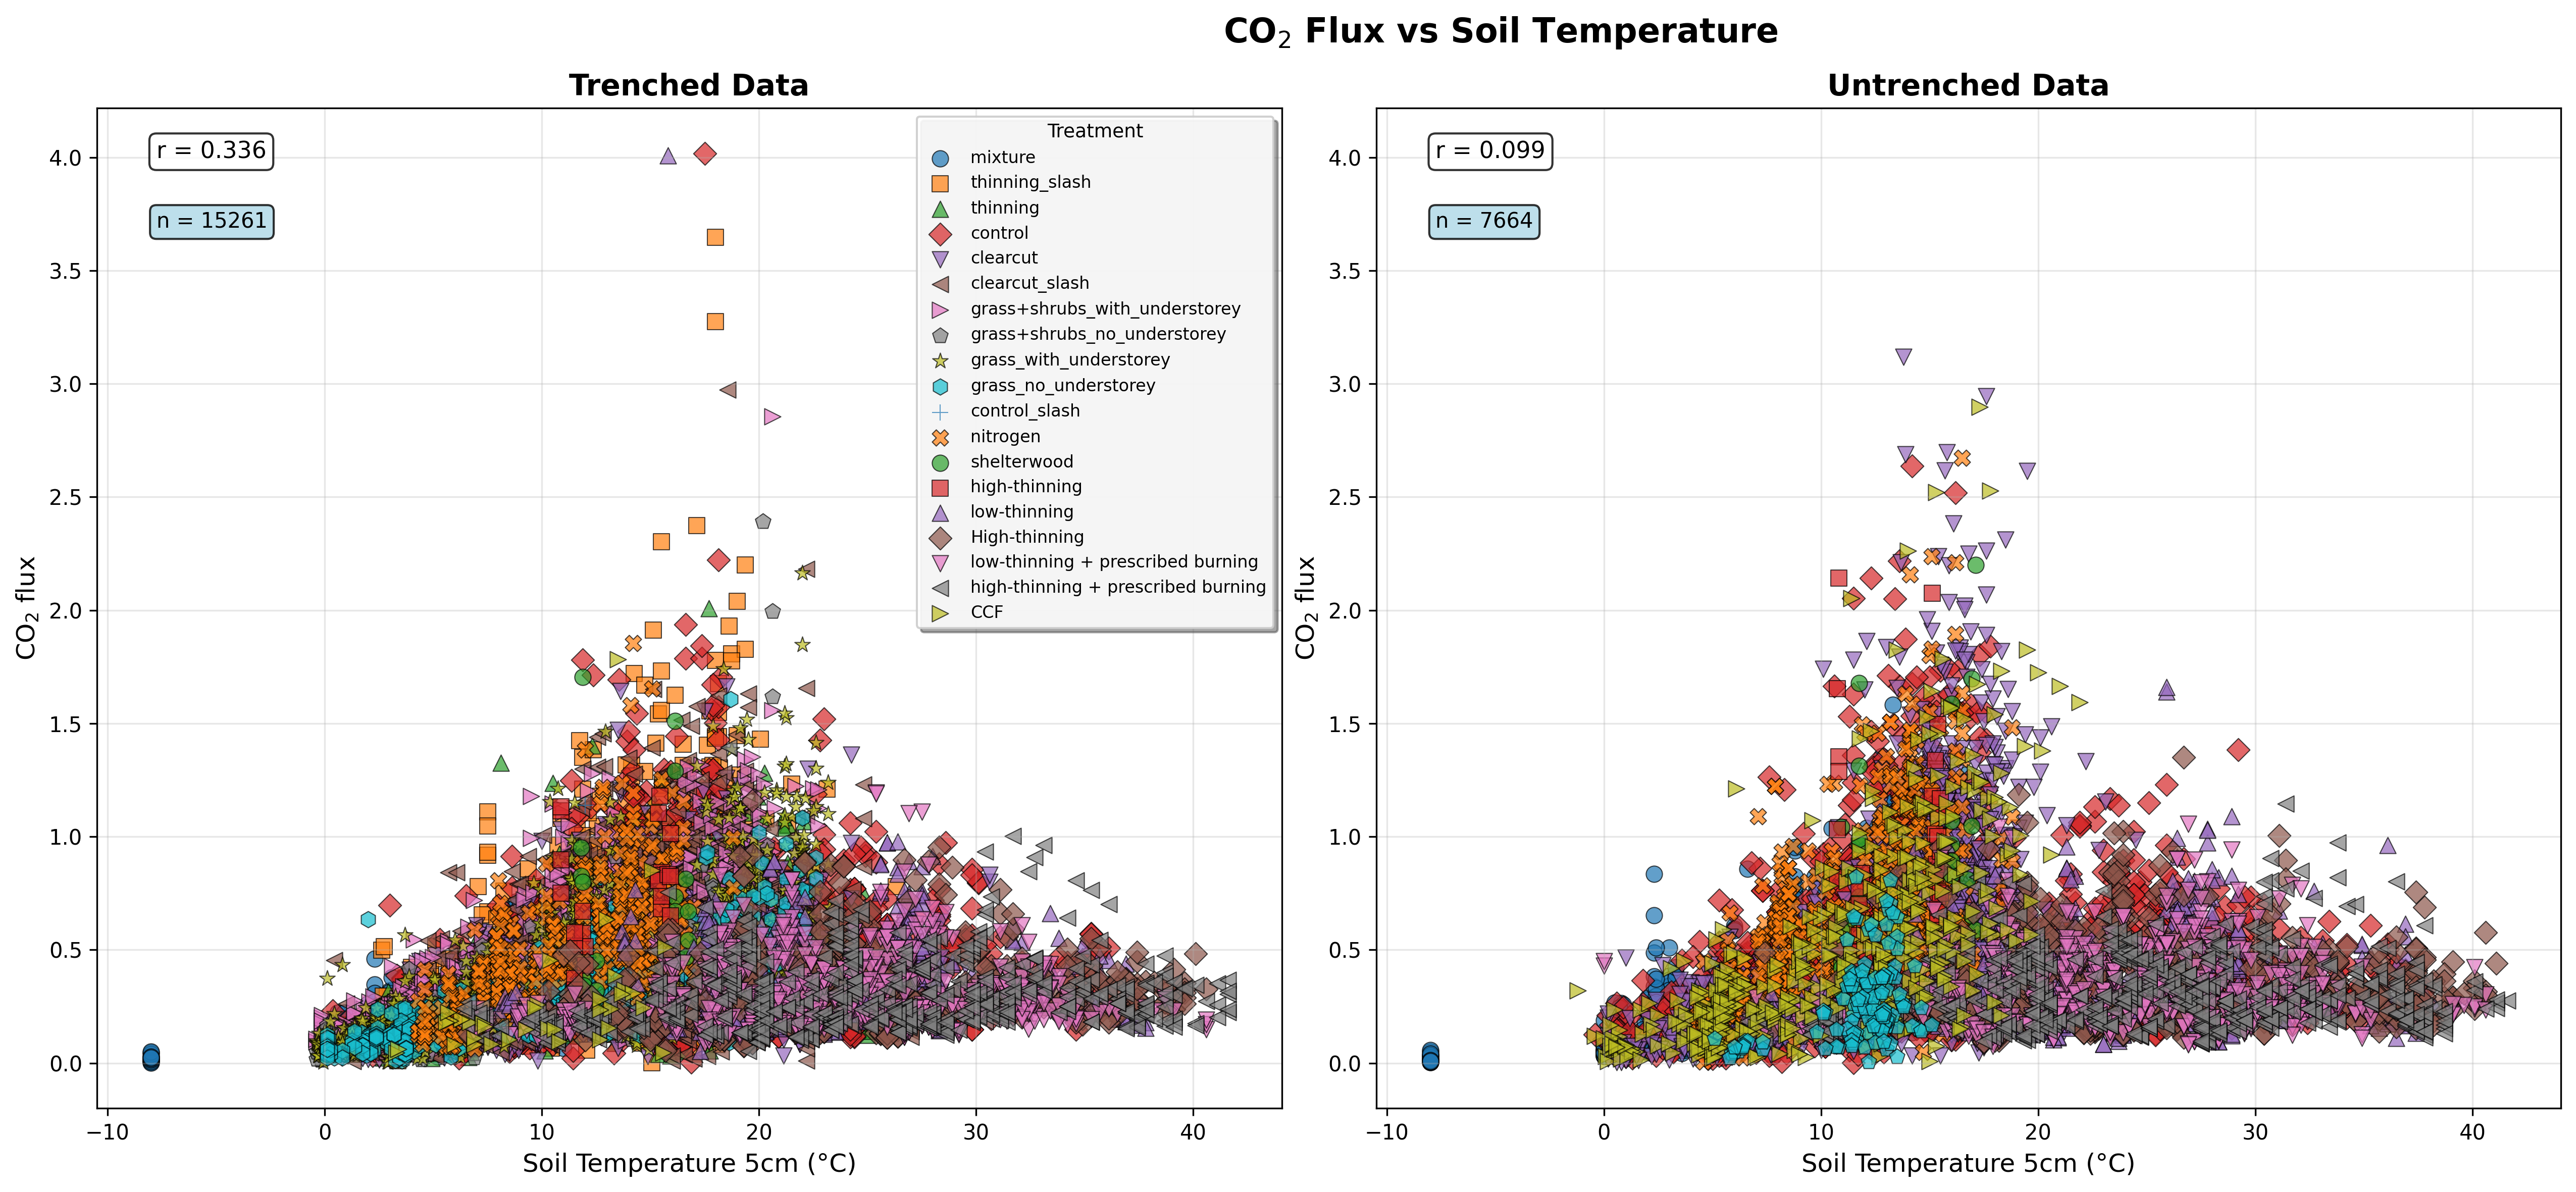
\includegraphics[width=0.8\textwidth]{"../co2_flux_temperature_comparison.png"}
    \caption{Example figure caption. Describe what the figure shows, including experimental conditions, sample sizes, and statistical tests. Error bars represent standard error of the mean. *p < 0.05, **p < 0.01.}
    \label{fig:example}
\end{figure}

\paragraph{Soil respiration and moisture}
% CO2 vs tmoisture
\begin{figure}[H]
    \centering
    \includegraphics[width=0.8\textwidth]{"../co2_flux_moisture_comparison.png"}
    \caption{Example figure caption. Describe what the figure shows, including experimental conditions, sample sizes, and statistical tests. Error bars represent standard error of the mean. *p < 0.05, **p < 0.01.}
    \label{fig:example}
\end{figure}

\paragraph{Moisture and temperature interactions}
% temperature vs tmoisture
\begin{figure}[H]
    \centering
    \includegraphics[width=0.8\textwidth]{"../soil_temperature_moisture_comparison.png"}
    \caption{Example figure caption. Describe what the figure shows, including experimental conditions, sample sizes, and statistical tests. Error bars represent standard error of the mean. *p < 0.05, **p < 0.01.}
    \label{fig:example}
\end{figure}


\paragraph{Autotrophic and heterotrophic fluxes}




\subsubsection{Modeling analysis}

% E_0 parameter
\begin{figure}[H]
    \centering
    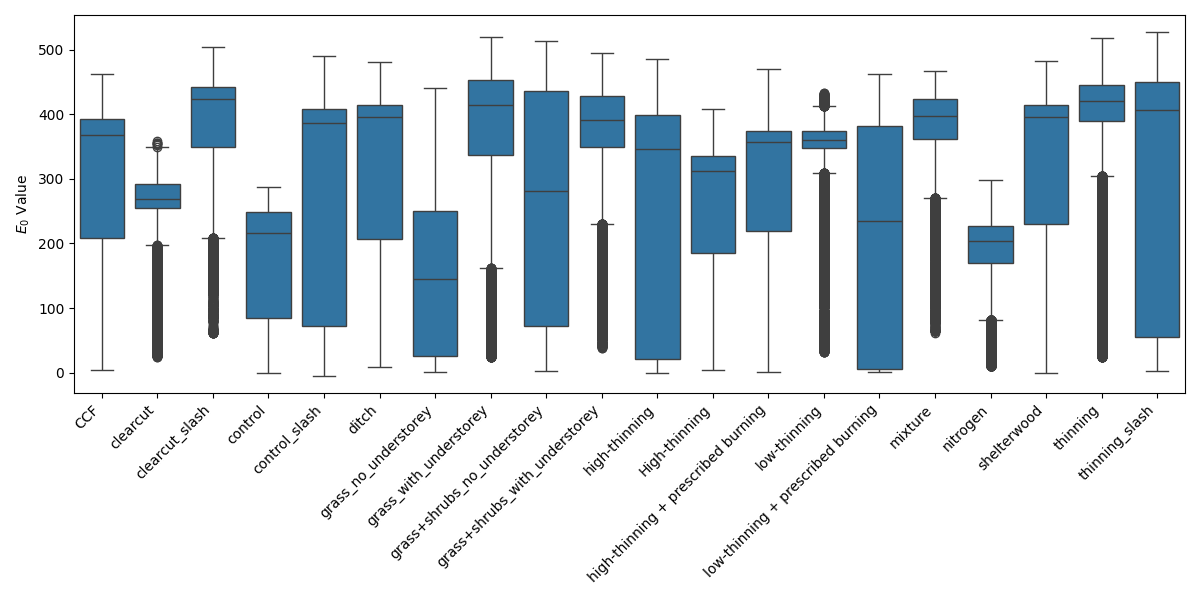
\includegraphics[width=0.8\textwidth]{"../ea_boxplot.png"}
    \caption{Example figure caption. Describe what the figure shows, including experimental conditions, sample sizes, and statistical tests. Error bars represent standard error of the mean. *p < 0.05, **p < 0.01.}
    \label{fig:example}
\end{figure}

% Other model params (except A)
\begin{figure}[H]
    \centering
    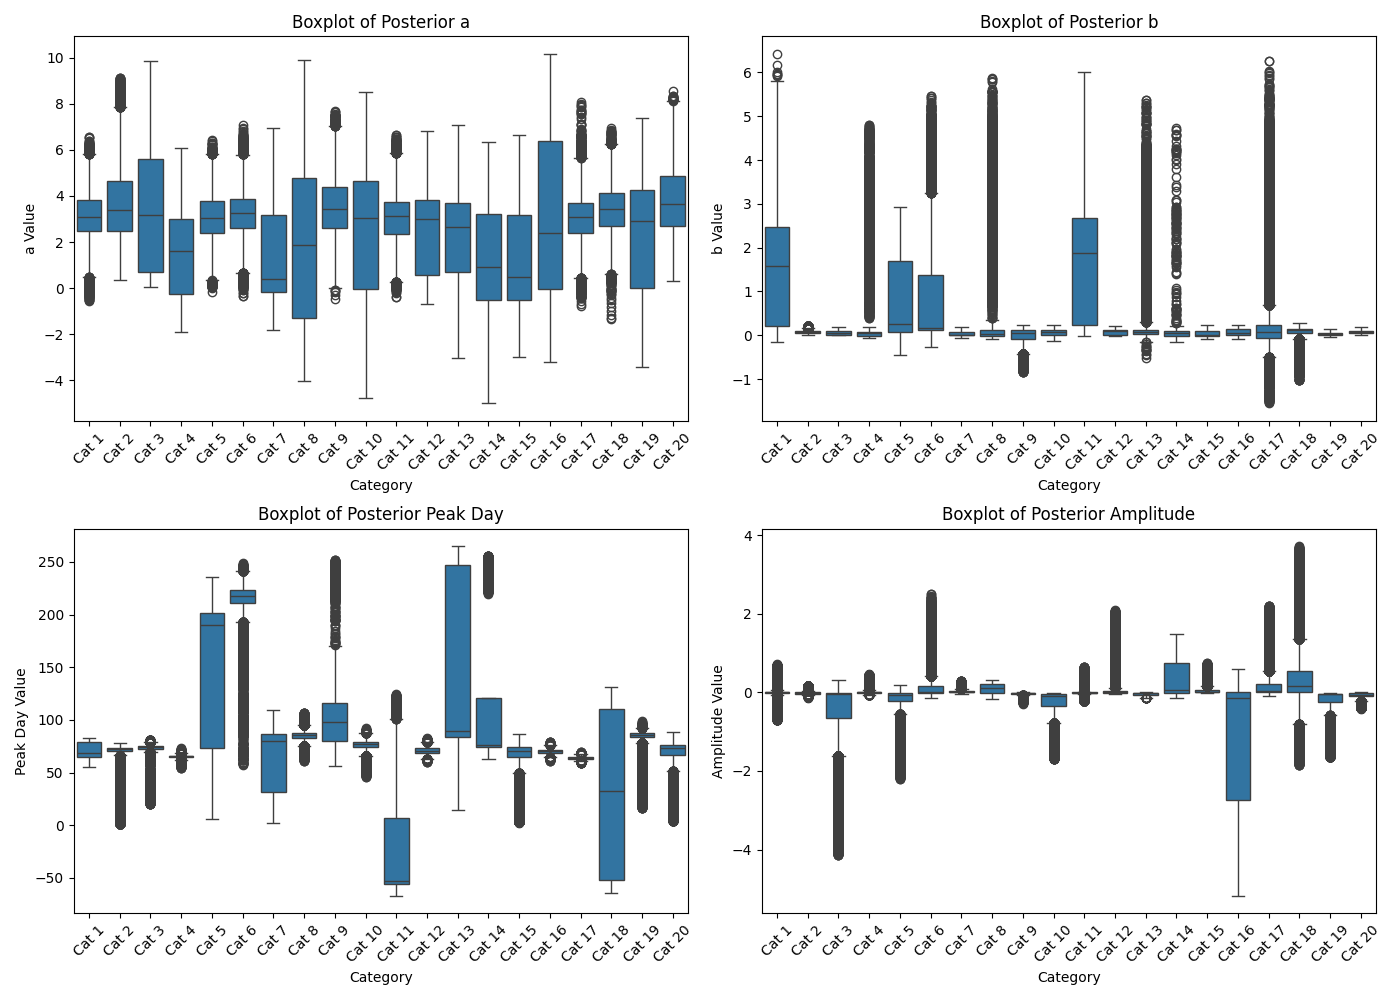
\includegraphics[width=0.8\textwidth]{"../other_params.png"}
    \caption{Example figure caption. Describe what the figure shows, including experimental conditions, sample sizes, and statistical tests. Error bars represent standard error of the mean. *p < 0.05, **p < 0.01.}
    \label{fig:example}
\end{figure}



\section{Discussion}

\subsection{Interpretation of Results}


\subsection{Limitations}

\subsection{Implications and Future Directions}



\section{Conclusions}

Summarize the key findings and their significance. Avoid simply repeating the abstract; instead, provide a synthesis that emphasizes the contribution of your work to the field.


\section*{Acknowledgments}

Acknowledge funding sources, institutional support, and individuals who contributed to the work but are not listed as authors.


\section*{Funding}

This work was supported by [Grant Agency] under Grant [Number]. [Author Name] was supported by [Fellowship/Scholarship].


\section*{Conflicts of Interest}

The authors declare no conflicts of interest.


\section*{Data Availability Statement}

The data that support the findings of this study are available from the corresponding author upon reasonable request [or specify repository/database where data are deposited].



% Bibliography
\bibliographystyle{plain}
\bibliography{references}


\end{thebibliography}

\end{document}